
\section{Electrocatalysis: An important piece of the answer}\label{sec:our_part}

In the last Section, I claimed that the most important remaining technological challenges that need to be solved to decarbonize society are (1) the intermittancy problem, which is to say the need to keep the lights on when the sun isn't shining and the wind isn't blowing, and (2) the electrification of other sectors.

\begin{figure}[h!]
	\centering
	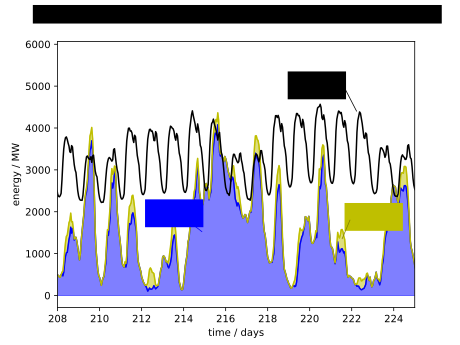
\includegraphics[width=0.7\textwidth]{01_Intro/fig/two_weeks_in_2017.png}
	\caption{The intermittancy problem. Electricity demand (black) compared to wind (blue) and solar (yellow) supply for Denmark over a two-week period in summer 2017. Data from \url{energinet.dk}, ref. \citen{EnergiNet}}
	\label{fig:intermittancy}
\end{figure}

The intermittancy problem becomes more important as the amount of intermittant renewable energy in a market increases. Figure \ref{fig:intermittancy} shows the electricity demand and intermittent renewable electricity generation in Denmark for a two-week period in the summer of 2017. Such datasets are available from \url{energinet.dk}. Overall, wind and solar met 45\% of electricity demand during that period, and wind and solar generation even exceeded demand for short periods of time. However, there were also periods of time, such as day 222-223, with little to no wind and solar, where all of Denmark's electricity generation came from bio and fossil fuels or from neighboring countries.

The following are some of the solutions most often proposed for the intermittency problem\cite{Budischak2013, Sgobbi2016, EU2018}:

\begin{itemize}
	\item Overcapacity of renewable generation, geographic diversification
	
	\item Flexible grid elements including battery vehicles
	
	\item \textbf{Hydrogen energy storage}
\end{itemize}

The first point is well under way, with cables linking Denmark's electricity network to the Swedish, Norwegian, and German grids, and cables planned to the Netherlands and Great Britain. Usually, the wind will be blowing or the sun shining in at least one of those places and, with enough wind generation overcapacity, that can help power neighboring regions. However, overcapacity is expensive, and there will still be times where demand is not met.

The second point involves utilizing market forces to get people to use electricity when it is most abundant. This could mean waiting until the wind is blowing and electricity is cheap to run a washing machine, or to charge a battery-powered vehicle. (Batteries are electrochemical devices, but out of the scope of this Thesis.) By extension, the varying price of electricity could even get people with battery vehicles to discharge their batteries when the wind isn't blowing, and so with sufficient electrification of transportation, the vehicle fleet could become a source of \textit{energy storage}. There are limitations in how far this can go: if every single car in Europe (300 million) was switched for an electric car with a typical car battery (30 kWh) and made fully accessible to the grid, this could power Europe (average 350 GW electricity in 2018) for 
\begin{equation}
\frac{3\cdot{10^8}\,\cdot\, 30 \text{[kWh]}}{350 \text{[GW]}} \approx 25 \text{[h]}\,,\nonumber
\end{equation}
or just about a day's electricity storage. Firstly, this is not enough energy storage to keep the lights on through a longer cloudy wind-still period. Secondly, most people will want to use their cars. Thirdly, full electrification of the personal vehicle fleet in Europe by 2030 is beyond any present ambition\cite{EU2018}, and it is hard to imagine total battery capacity growing faster in any other sector. So, while batteries will help, they are not the full answer.

The last point, in bold, depends on electrochemical technologies - water \textit{electrolyzers} which use electrochemical energy to split water into hydrogen and oxygen; and hydrogen \textit{fuel cells} which generate electrical energy by the reaction of hydrogen and oxygen. Electrolyzers are described in more detail below.

%\begin{figure}[h!]
%	\centering
%	\includegraphics[width=0.7\textwidth]{01_Intro/fig/Seh.png}
%	\caption{A sketch of renewable energy infrastructure and chemical industry with electrocatalysis at the center. By Jakob Kibsgaard, in Seh et al, 2017, ref. \citen{Seh2017}.}
%	\label{fig:Seh}
%\end{figure}

%Figure \ref{fig:Seh} by Jakob Kibsgaard in ref. \citen{Seh2017} shows a diagram of energy and material flows in a society that has implemented the answer to question \ref{q:how} in the previous Section, with emissions reductions accomplished by renewable electricity and by electrification of transport and industry. The intermittency problem has been solved by hydrogen energy storage.
\vspace{5mm}
The following have been proposed as means to electrify other sectors\cite{EU2018}:
\begin{itemize}
	\item Buildings\cite{David2017}: replace fuel heating with electric heat pumps
	
	\item Transport \cite{Cano2018, Thiel2016}:
	\begin{itemize}
		\item more reliance on electric-powered mass transit
		
		\item battery-electric vehicles, mainly for personal vehicles
		
		\item \textbf{hydrogen fuel cell vehicles}, mainly for buses \& trucks, etc
		
		\item Eventually \textbf{Use electrical energy to make fuels} for heavy transport
	\end{itemize}

	
	\item Industry \cite{Lechtenbohmer2016}:
	\begin{itemize}
		
		\item Replace fuel heating with electrical heating. 
		
		\item When possible, replace fossil fuel reactants with \textbf{electrochemically produced hydrogen}.
		
		\item
		When possible, \textbf{replace thermal processes with electrochemical processes}. 
		
	\end{itemize}
\end{itemize}

The points in bold depend on a number of electrochemical technologies, some mature and some emerging. One clear aspect is the central role of electrochemically generated hydrogen, not only for energy storage in the electrical grid, but also as a renewable energy input in other sectors. 
I will briefly describe the water electrolyzers used for electrochemical hydrogen production, and then mention some of its uses and some of the other electrochemical processes of interest for decarbonizing transport and industry.

\vspace{5mm}
Hydrogen (\ch{H2}) can be produced electrochemically by electrolysis of water (\ch{H2O}) into oxygen (\ch{O2}) and \ch{H2}. The overall reaction is:
\begin{equation}
\ch{2 H2O -> 2 H2 + O2}\label{rxn:split}
\end{equation}
It is actually extremely simple to drive this reaction (inefficiently) with electrical energy. One need only tape wires to the two ends of a four-volt battery, and then put the wires in a cup of salt water. Bubbles will develop on both wires. The bubbles on the wire connected to the positive end of the battery (the anode) are \ch{O2}, and the bubbles on the wire connected to the negative end of the battery (the cathode) are \ch{H2}. The reaction is separated into \textit{anodic} and \textit{cathodic} reactions, the first of which involves \textit{oxidizing} water to \ch{O2}, and the second of which involves \textit{reducing} water to \ch{H2}. These two reactions, referred to, respectively as the oxygen evolution reaction (OER) and hydrogen evolution reaction (HER) are written as follows:
\begin{align}
\ch{2 H2O &-> O2 + 4 (H+ + e- )} &&\text{OER}\label{rxn:OER}\\
\ch{2 (H+ + e- ) &-> H2} &&\text{HER}\label{rxn:HER}
\end{align}
They are connected by \textit{electrons} (\ch{e-} ) flowing through the wires and the power source, and by \textit{protons} (\ch{H+}) or other charge carriers moving through the liquid, which is therefore called an \textit{electrolyte}. The voltage between the anode and cathode, called the \textit{cell potential}, is what drives the reaction. It makes the electron energy lower on the anode and higher on the cathode, pushing both reactions, as written here, in the forward direction. 

How much do we need to push the electrons? There is a minimum, 1.23 V, which is set by the thermodynamics of Reaction \ref{rxn:split}, but in practice it will always require more. It costs some potential - the electrical current times the \textit{solution resistance} - to push the ions between the anode to the cathode. It also costs some potential to drive reactions \ref{rxn:OER} and \ref{rxn:HER} themselves. This potential, called the \textit{catalytic overpotential} and depends on the electrode material.A material that minimizes the overpotential is a good \textit{electrocatalyst}.

\begin{figure}[h!]
	\centering
	\includegraphics[width=\textwidth]{01_Intro/fig/electrolyzers.png}
	\caption{Schematic diagrams of the three types of water electrolyzer cells: Alkaline electrolysis cell (AEC), polymer electrolyte membrane electrolysis cell (PEMEC), and solid oxide electrolysis cell (SOEC). From ref. \citen{Schmidt2017}.}
	\label{fig:electrolyzers}
\end{figure}

Three designs for \textit{water electrolyzers} producing hydrogen from water by Reactions \ref{rxn:OER} and \ref{rxn:HER} are shown in Figure \ref{fig:electrolyzers}, from ref. \citen{Schmidt2017}. For detailed discussion and comparison of these technologies, I refer the reader to a number of excellent reviews, assessments, and perspectives including refs. \citen{Schmidt2017, Xiang2016, Bhandari2014, Buttler2018, Zeng2010, Carmo2013, Babic2017, Chen2016b}. Briefly, the three technologies differ fundamentally in the type of electrolyte (indicated in \textbf{bold}) and electrocatalyst (in \textit{italics}) used: 

\begin{itemize}
\item Alkaline electrolysis cells (AEC's) are the electrolyzers most in use today, and the type that most resemble the wires-in-a-glass setup described above. In an AEC, the anode and cathode are immersed in an electrolyte of \textbf{concentrated alkaline solution}. The charge is carried by hydroxide ions through a porous ceramic called the separator. The separator's purpose is to keep the \ch{H2} from the cathode and \ch{O2} from the anode separate, but a small amount of \ch{H2} will diffuse over to the anode side. This is the main drawback of AEC's: they must be run at high current density to avoid making an explosive mix of \ch{O2} and \ch{H2}. This makes them less than ideal for solving the intermittancy problem. Another drawback is a high solution resistance. The main advantage, as will be described in more detail at the start of Chapter \ref{ch:O2}, is that there are cheap electrode materials that can catalyze Reactions \ref{rxn:OER} and \ref{rxn:HER} in alkaline electrolyte. \textit{Nickel} works reasonably well for both electrodes.

\item Polymer electrolyte membrane electrolysis cells (PEMEC's) utilize a proton-conducting \textbf{polymer electrolyte membrane} such as the commercial Nafion from DuPont. The main advantages are that the resistance to proton transport across the membrane is very low while the membrane is very effective at blocking gas crossover. The disadvantage, as will be described in more detail at the start of Chapter \ref{ch:O2}, is that the membrane is in effect a very acidic electrolyte, and that there are at present no cheap and stable electrocatalysts that can facilitate Reactions \ref{rxn:OER} in acid. Present PEMEC's use \textit{platinum at the cathode and iridium and/or ruthenium oxides at the anode}. These are all very rare metals.

\item Solid oxide electrolysis cells (SOEC's) are an up-and-coming technology. Here the electrolyte is a solid \textit{\textbf{oxide-conducting ceramic}} such as yttrium-stabilized zirconia (YSZ), which transports oxide anions (\ch{O^{2-}}) at high temperature. The disadvantage is that they have to run at very high temperature, on the order of 800$^\circ$C, at which the materials degrade. The advantage is that there is little to no catalytic overpotential on the oxide itself at these temperatures, and so water splitting is done with very high energy conversion efficiency.
\end{itemize}

PEMEC's are expected by many experts to be the predominant water electrolysis technology by 2030, as hydrogen begins to play an important role in decarbonization\cite{Schmidt2017}. Their domanince increases if more efficient and scalable electrocatalysts are developed. This is the main motivation for the materials of study in the Chapters of this Thesis. Most of the experiments presented in Chapter \ref{ch:Tools}, though used primarily to characterize the experimental techniques, are done on platinum, which is used on the cathode of PEMEC's. Most of the experiments presented in Chapter \ref{ch:O2} are done on ruthenium dioxide (\ch{RuO2}), which is a catalyst material for the anode of PEMEC's.

%\begin{figure}[h!]
%	\centering
%	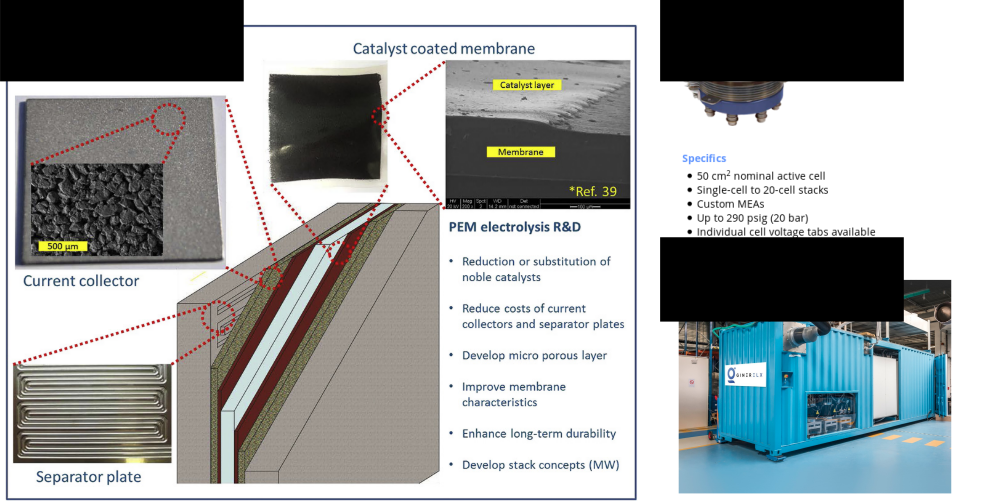
\includegraphics[width=\textwidth]{01_Intro/fig/PEM_electrolyzers.png}
%	\caption{}
%	\label{fig:PEM}
%\end{figure}
\vspace{5mm}
Electrochemically generated hydrogen can be stored in tanks, and used in any of the following ways:
\begin{itemize}
	\item Electricity generation for the grid via a fuel cell. The dominant fuel cell technology today is a polymer electrolyte membrane fuel cell (PEMFC), which is the PEMEC of Figure \ref{fig:electrolyzers} in reverse, with a platinum catalyst on the oxygen side\cite{Debe2012}. Solid oxide fuel cells are an emerging technology.
	
	\item Transport in PEMFC electric vehicles.
	
	\item Reduction of iron ore for steel production.  At present, steel is produced by the approximate reaction:
	\begin{equation}
	\ch{2 Fe2O3 + 6 C + 3 O2 -> 2 Fe2O3 + 6 CO -> 12 CO2 + 4 Fe}\,, 
	\end{equation} 
	The stoichoimetric carbon from this reaction accounts for more than 3\% of global \ch{CO2} emissions (Paper \ref{Nitopi2019}).
	
	An emerging steel-making process\cite{Fischedick2014} uses direct reduction by \ch{H2} instead:
	\begin{equation}
	\ch{Fe2O3 + 3 H2 -> 3 H2O + 2 Fe}
	\end{equation}
	In some models of the future energy+industrial landscape, this will be the primary use of renewable hydrogen in 2030 and beyond\cite{Sgobbi2016}.
	
	\item The Habor-Bosch process which makes ammonia for fertilizer: 
	\begin{equation}
	\ch{N2 + 3 H2 -> 2 NH3}
	\end{equation}
	At present, the hydrogen used in this process comes from steam reforming of natural gas:
	\begin{equation}
	\ch{CH4 + 2 H2O -> 4 H2 + CO2}
	\end{equation}
	The stoichiometric amount of carbon used in steam reforming for ammonia production today is about 0.5\% of global \ch{CO2} emissions (Paper \ref{Nitopi2019}).
	
	\item Production of liquid fuels by the reaction of \ch{H2} and \ch{CO2} captured from point sources or the air. This involves first producing syngas, a combination of \ch{CO} and \ch{H2}, by reacting an excess of \ch{H2} with \ch{CO2} by the water-gas shift reaction, and removing the water:
	\begin{equation}
	\ch{H2 + CO2 -> H2O + CO}
	\end{equation}
	Syngas can be used to synthesize methanol or long-chain hydrocarbons (Fischer-Tropsch reaction) depending on the catalyst and reaction conditions\cite{Concepts2003}.
\end{itemize}

\begin{figure}[h!]
	\centering
	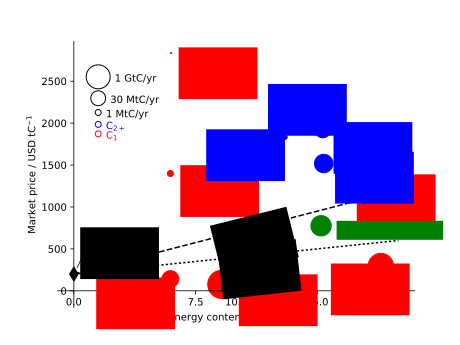
\includegraphics[width=0.7\textwidth]{01_Intro/fig/carbon_products.png}
	\caption{Mapping of fuels and chemicals comparing market price with minimum cost of electricity and \ch{CO2} for two different electricity prices. The size of each dot indicates the market size, on a log scale. All quantities are normalized to mass of carbon. Adapted from Paper \ref{Nitopi2019}. Jet fuel has been added assuming the carbon density and energy content of decane (\ch{C10H22}).}
	\label{fig:products}
\end{figure}

With respect to the last point above, it is interesting to ask: 
\begin{question}
	What products would be smart to make by using renewable energy to convert \ch{CO2}?
\end{question}
Figure \ref{fig:products} is a generalized and simplified approach to answering that question. It shows the market price vs the energy content for a number of carbon products, with the size of the marker representing the market size. The lines represent the minimum cost to make a product given prices for the \ch{CO2} starting material and the renewable electricity. Products above the line might be economically viable, while products below the line can not be. In Paper \ref{Nitopi2019}, we use this analysis to motivate the production of ethylene (Reaction \ref{rxn:etOH}) and ethanol (Reaction \ref{rxn:C2H4}) by direct electrochemical \ch{CO2} reduction on copper electrodes:
\begin{align}
\ch{2 CO2 + 12 (H+ + e- ) &-> C2H4 + 4 H2O}\label{rxn:etOH}\\
\ch{2 CO2 + 12 (H+ + e- ) &-> CH3CH2OH + 3 H2O}\label{rxn:C2H4}
\end{align}
This reaction has also been a focus of my PhD (Papers \ref{Scott2019_GIXRD}, \ref{Nitopi2019}, and \ref{Scott_Engstfeld2019}), though not the Chapters of this Thesis.

Because it is only based on thermodynamics, the economic argument in Figure \ref{fig:products} is equally valid with thermal reaction of \ch{CO2} with \ch{H2} produced by electrolysis with renewable electricity. I have added a possible Fischer-Tropsch reaction product, decane (\ch{C10H22}), which is representative of heavy transport fuel (aviation fuel is primarily hydrocarbons of length 5-15). This product is not thermodynamically impossible to make at the present market price with electricity at 20 USD per MWh (near the record lows for solar installations), but is impossible at 50 USD per MWh (more typical of present solar installations). It is very important to realize, though, that the actual cost of making a product will be significantly higher than the lines in Figure \ref{fig:products} because of overpotentials, capital costs, and other operating costs.

The price of captured \ch{CO2} in Figure \ref{fig:products}, USD 200 per ton of carbon, is representative of carbon captured from a power plant\cite{Majumdar2016}. Carbon captured from the air would be much more expensive, pushing the lines up. A carbon tax, however, would push the lines down, since captured and utilized \ch{CO2} avoids the tax. This is clearly essential if renewable fuels are ever going to compete with the likes of coal and natural gas.


\vspace{5mm}
To conclude this Chapter, before diving into the heavy electrocatalysis of this Thesis, I should introduce one essential aspect in the study of electrochemistry, the \textit{three-electrode setup}. A more complete introduction to electrochemistry\cite{Bard2001, Scott2016_MSc} is beyond the scope of this Thesis, but with this one concept, a new reader might be able to follow the experiments in the next Chapters, which attempt to introduce other new concepts as they come up.

\begin{figure}[h!]
	\centering
	\includegraphics[width=0.5\textwidth]{01_Intro/fig/3E.png}
	\caption{Diagram of the three-electrode setup. The dotted-line box at the top represents a potentiostat. From my master's thesis, ref. \citen{Scott2016_MSc}.}
	\label{fig:3E}
\end{figure}

When running an electrochemical process in industry, there is typically only one potential difference that matters: the cell potential between the anode and the cathode. This potential difference, times the current, is the power being consumed. However, in electrocatalysis research, it is almost always preferable to study the anode or cathode reaction in isolation. 

This means, most often, controlling the potential of the sample, referred to as the \textit{working electrode} (WE), on an absolute scale while measuring the current passing through it. The absolute potential scale is accomplished by using a \textit{reference electrode} (RE), which contains each of the reactants and products in a facile redox reaction at steady, well-defined activities. The reference electrode used for the experiments in this Thesis is a mercury/mercury sulfate reference electrode, based on the redox reaction
\begin{equation}
\ch{Hg + SO4^{2-} <-> HgSO4 + 2 e-}
\end{equation}
Since Hg and \ch{HgSO4} are solids, only the activity of \ch{SO4^{2-}} can potentially vary. It is kept constant by using a saturated \ch{K2SO4} solution. The \textit{equilibrium potential} of such a reaction is a constant value determined by thermodynamics, so as long as there is no current flowing through the reference electrode (above the tiny current that a voltmeter uses to measure a potential difference).

The absolute potential of the WE is determined on the scale of the RE just by measuring the potential difference between them with a voltmeter. Controlling the potential is a bit trickier. The way to change the potential of the WE is actually to run a current through it. This charges the electrode-electrolyte interface, which is what determines the electrochemical potential. But running a current through the RE isn't an option, because then the redox reaction would no longer be at equilibrium and the potential would no longer be well defined. So we need a third electrode, called the \textit{counter electrode} (CE) who's only purpose is to conduct the current needed to get the working electrode to the desired potential. The current through the CE is equal and opposite to the current through the WE.

So, to get the WE to a desired potential vs the RE, what actually happens is that a voltage is set between the WE and the CE, and the resulting current changes the absolute potential of the WE, which is measured against the RE, and this is iterated until the WE is at the requested potential against the RE. Then, the current is measured. This is often done while scanning the WE potential back and forth smoothly to measure the current as a function of the linearly changing potential, a technique called \textit{cyclic voltammatry}. Doing this smoothly requires some fancy electronics, and the machine containing these electronics is called a \textit{potentiostat}. This setup is shown in Figure \ref{fig:3E}.

So that's how we study one electrode material at a time. But you may notice that the only information we get from the potentiostat is the electrochemical current and potential. You may be wondering,
\begin{question}
	How do we know which reaction(s) the current is going to?
\end{question}
That is the right question to bring us to the next Chapter.


